%!TEX root = kPtx_paper.tex
\section*{Methods}
\subsection*{Design and Simulation Setup}
Simulations were performed to validate and characterize the proposed k-space domain parallel transmit pulse design method,
with comparisons to the spatial-domain method of Ref. \cite{Grissom:2006:MRM}.
RF pulses were designed for a simulated 24-channel loop transmit array (Figure \ref{fig:Coil}) that is being built for a 7 Tesla scanner optimized
for imaging the human cortex.  
24-channel complex-valued $B_1^+$ maps used in the pulse designs were simulated in a male human head model using 
Ansys High Frequency Structure Simulator (Canonsburg, PA, USA) with 1.5 mm isotropic resolution. 
Figure \ref{fig:Target}a shows the target pattern for all pulse designs which comprised an ellipse centered on the ventricles with AP/HF/LR semi-axes of 4.8/3.2/3.2 cm.
The pattern was smoothed by a Fermi filter that was applied in the frequency domain to match the target pattern's effective resolution to the excitation k-space trajectory's 5 mm resolution.
This choice of target pattern was motivated by imaging applications for the 7 Tesla scanner 
in which midbrain signals will be saturated for high-resolution, highly-accelerated imaging of the cortex. 
Pulses were designed to excite the entire ellipse and achieve zero excitation in voxels in the cerebrum but outside the ellipse. 
The smoothed target pattern and the $B_1^+$ maps were downsampled from their original 128$\times$128$\times$96 grids (1.5 mm isotropic resolution) to 
64$\times$64$\times$48 grids (3 mm isotropic resolution),
and RF designs were performed with the 64$\times$64$\times$48 grid size. 


\begin{figure}
	\centering
	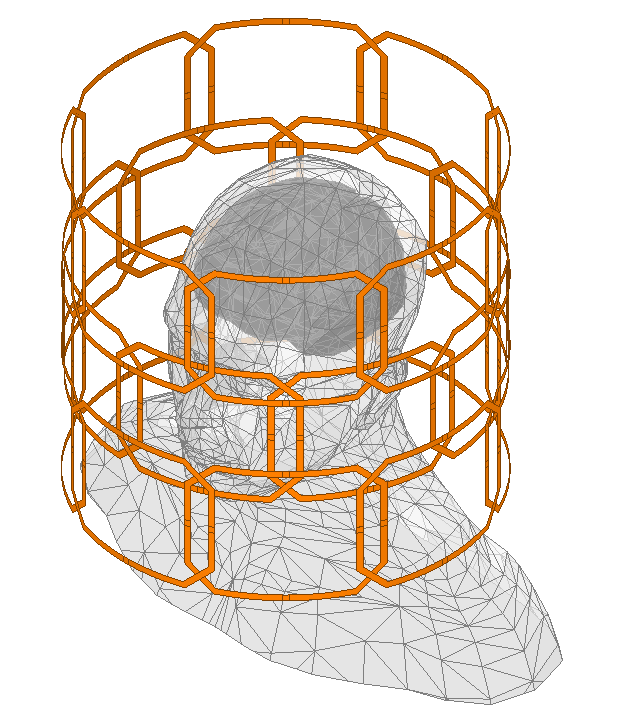
\includegraphics[width=6cm]{kspace_PTX_Coil}
	\caption{The 24-channel loop Tx array that was simulated in a human head model to obtain $B_1^+$ maps. 
	The array has diameter 32 cm and height 28 cm. The 16 cm $\times$ 11 cm rectangular loops are arranged in 3 rows of 8.}
	\label{fig:Coil}
\end{figure}

\par A SPINS excitation k-space trajectory \cite{malik2012tailored} (Figure \ref{fig:Target}b) with 5 mm max resolution was used for the designs. 
The SPINS trajectory comprised three segments with radii ranging between 1-0.625, 0.625-0.375, and 0.375-0 cycles/cm, respectively.
The number of polar and azimuthal rotations were 15.5/2.125, 20.66/2.833, 15.5/2.125 for each segment, respectively.
The SPINS trajectories were first designed analytically and the final gradient waveforms and excitation k-space trajectories were designed from them 
using the minimum-time gradient waveform design method \cite{lustig2008fast}, 
for a 15 {\textmu}s dwell time and subject to the scanner's gradient amplitude and slew rate constraints of 200 mT/m and 700 T/m/s, respectively (Figure \ref{fig:Target}c). 
The durations of the three segments after minimum-time gradient design were 4.174, 4.326, and 1.5 ms, respectively.
With the exception of the simulations across undersampling factors, 
all pulse designs used this 10 ms trajectory.
With this trajectory and the 64$\times$64$\times$48 design grid size, 
the dimensions of the $\bm{W}$ matrix were 16,632 RF pulse samples, by 196,608 target k-space locations. 

\begin{figure}
	\centering
	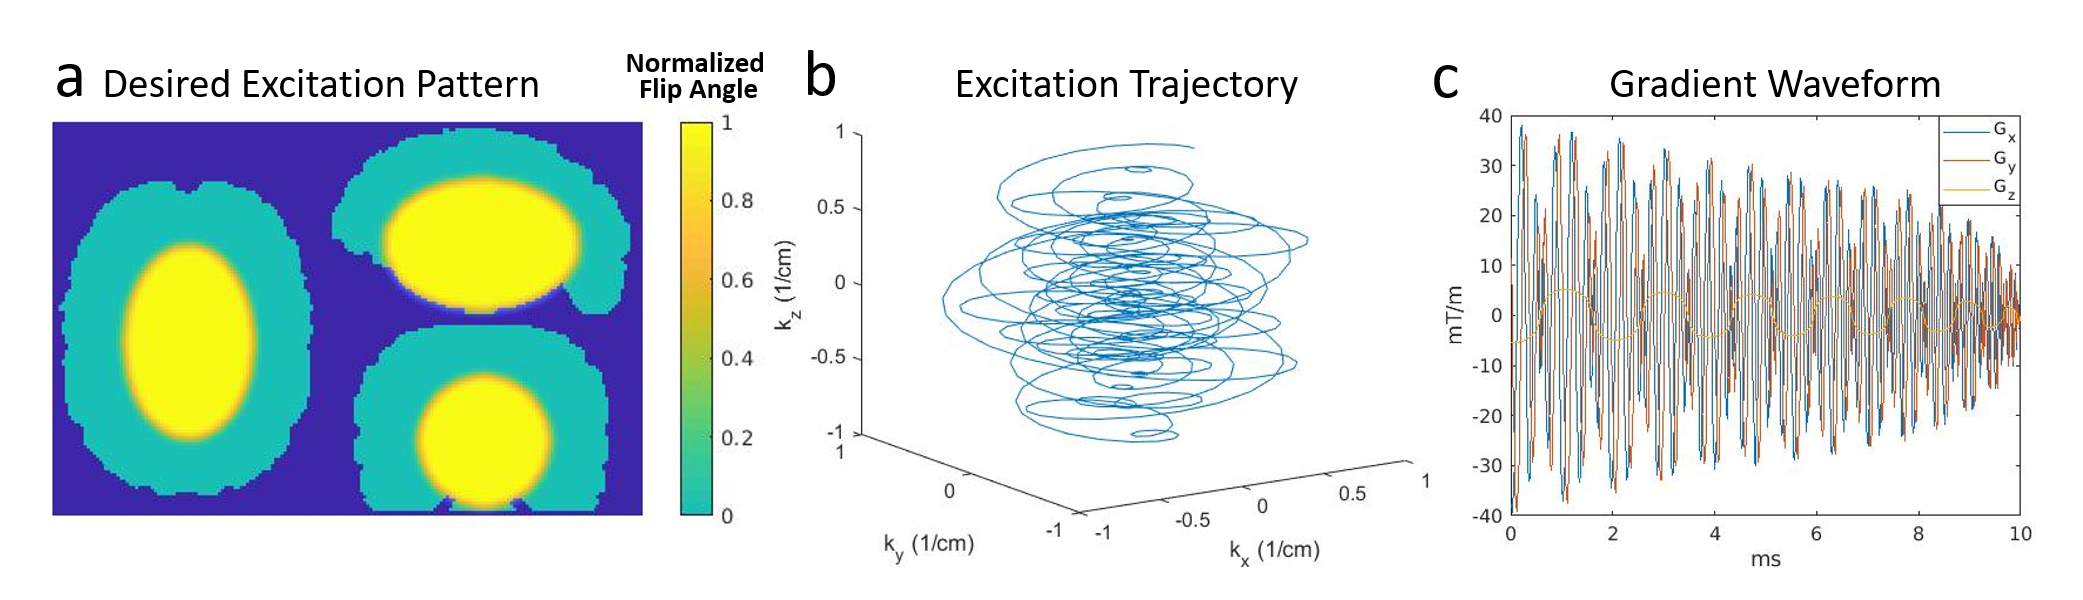
\includegraphics[width=\textwidth]{kSpace_PTX_Pattern_Trajectory}
	\caption{(a) Middle axial, sagittal, and coronal slices of the target excitation pattern used for all pulse designs. 
	(b) The SPINS trajectory used in the designs. 
	(c) 10 ms minimum-time gradient waveforms that produce the SPINS trajectory.}
	\label{fig:Target}
\end{figure}

\par All pulse designs and Bloch equation simulations were performed in MATLAB (Mathworks, Natick, MA, USA).
For spatial domain designs, 
RF pulses were solved using an iterative least-squares conjugate-gradient descent method \cite{Grissom:2006:MRM} with 35 iterations,
which was accelerated by non-uniform fast Fourier transforms \cite{Fessler:2003fk}. 
Except for the off-resonance-compensated designs described below, 
all spatial domain designs were parallelized using 16 threads that simultaneously computed the forward and backward 
non-uniform fast Fourier transforms across transmit coils. 
The proposed k-space domain algorithm was implemented based on code for the non-Cartesian GRAPPA method of Ref. \cite{luo2019grappa},
as a function that takes as input the $B_1^+$ maps, 
a normalized excitation k-space trajectory, and optional structures of algorithm and off-resonance parameters. 
Within that function the Fourier transforms of the $B_1^+$ products are calculated,
and a C-based MEX function is invoked to solve for the non-zero elements of each column of $\bm{W}$,
with linear interpolation of the Fourier transforms of the $B_1^+$ map products to obtain the entries of the $\bm{S}^H\bm{S}$ matrices. 
Those elements are then inserted into a sparse $\bm{W}$ matrix, which is the single output of the main function. 
Parallelization was implemented across patches within the C-based MEX function using OpenMP. 
The final pulses are calculated by multiplying the sparse $\bm{W}$ matrix into the Fourier transform of the target pattern. 
This code, the $B_1^+$ maps, and a demo script are available at https://github.com/wgrissom/kpTx. 
All pulse designs were performed on a server (Colfax International, Santa Clara, CA, USA) 
with 512 GB RAM and two 24-core 2.1 GHz Intel Xeon CPUs which provide up to 94 threads (Intel Corporation, Santa Clara, CA, USA). 
Designs were performed five times for each case, and the mean computation time was recorded.
For the k-space domain designs, the design time comprised the time to compute the sparse $\bm{W}$ matrix, 
and the time to multiply it into the target pattern to obtain the pulses.
The resulting pulses were Bloch equation-simulated and compared to the target pattern on the finer 128$\times$128$\times$96 grid to capture Gibbs ringing. 
When calculating excitation errors, the magnitude root-mean-square error (RMSE) was calculated in voxels within the cerebrum,
except for an $\approx$5 mm-thick transition band around the edge of the elliptical target region.

\subsection*{k-Space Algorithm Parameters}
To evaluate how accuracy and compute time depend on k-space-domain design parameters and parallelization,
pulse designs were done across numbers of threads (i.e., how many patches were solved simultaneously; 1 to 32), 
patch widths (1 to 16 cycles/FOV), and inclusion widths (2 to 8 cycles/FOV). 
The number of threads were varied while holding the patch width and inclusion width both at 4 cycles/FOV.
The patch width was varied while holding the number of threads at 16, and the inclusion width at 4 cycles/FOV,
and the inclusion width was varied (2, 4, 6, and 8 cycles/FOV) while holding the number of threads at 16, and the patch width at 4 and 8 cycles/FOV. 
The sizes of the $\bm{W}$ matrices were also recorded, holding patch width constant at 4 cycles/FOV and varying the inclusion width. 

\subsection*{L-Curves}
To compare the tradeoff between excitation error (measured by root-mean-square error)
and integrated RF root-mean-square (RMS) amplitude for spatial and k-space domain designs,
pulse designs were repeated while varying Tikhonov regularization parameters ($\lambda$ in Equation \ref{eq:Solution}) 
over five orders of magnitude. 
The k-space domain designs were repeated four times to investigate the three main sources of error:
finite patch width, finite inclusion width, and $B_1^+$ map product interpolation. 
Specifically, a design was performed using patch and inclusion widths of four
with interpolated $B_1^+$ map products (`Interpolated $\bm{S}^H\bm{S}$ matrices'),
patch and inclusion widths covering the entire design grid with interpolated $B_1^+$ map products,
patch and inclusion widths of four without $B_1^+$ map product interpolation (`Exact $\bm{S}^H\bm{S}$ matrices'; 
$B_1^+$ maps were phase-modulated to each trajectory location before Fourier transform),
and patch and inclusion widths covering the entire design grid without $B_1^+$ map product interpolation. 
Note that the last case is equivalent to the original k-space domain method of Ref. \cite{Katscher:2003:Magn-Reson-Med:12509830}.
For each design, flip angle RMSE (calculated using the spatial domain non-uniform fast Fourier transform) and root-mean-square RF amplitude was
calculated.

\subsection*{Gibbs Ringing}
Gibbs ringing commonly arises in spatial domain parallel pulse designs when the resolution of the 
design grid is similar to that of the excitation k-space trajectory. 
The proposed k-space-domain method is implemented without wraparound or circulant end conditions in excitation k-space, 
so Gibbs ringing should be suppressed even when using a design grid that is only slightly wider than the trajectory. 
To demonstrate this, 
the target pattern and $B_1^+$ maps were further down-sampled to 32$\times$32$\times$24 (6 mm isotropic-resolution),
and the outermost leaves of the SPINS trajectory which had duration 2.1 ms were excluded so that the maximum excitation 
resolution matched the 6 mm target pattern and $B_1^+$ map resolution. 
Pulses were designed by the spatial domain method using both 32$\times$32$\times$24 and 64$\times$64$\times$48 grid sizes,
and by the k-space-domain method for 32$\times$32$\times$24 grid size.
The designed pulses were then evaluated against the target pattern using the 128$\times$128$\times$96 grid size,
to visualize the ringing.

\subsection*{Excitation k-Space Undersampling}
An important application of parallel transmission is the reduction of multidimensional pulse durations by excitation k-space undersampling.
To compare the spatial domain and k-space domain methods across undersampling factors,
the number of polar and azimuthal rotations were increased and reduced relative to the reference design described above, 
for reduction factors of 0.5, 2, 3, and 4. 

\subsection*{Off-Resonance}
To compare the off-resonance-compensated k-space domain designs with off-resonance-compensated spatial domain designs,
we incorporated a Gaussian ($\sigma = 3$ cm) field map centered above the frontal sinus, 
which was designed to mimic the characteristic susceptibility-induced $B_0$ inhomogeneity in this part of the human brain. 
The field maps were than scaled so that the maximum off-resonance reached +200 Hz and +400 Hz.
A time-segmented approximate off-resonance model was calculated using the method of Ref. \cite{fessler2005toeplitz} with $L = 4$ time segments,
and this model was used in both spatial domain and k-space domain designs. 
Both spatial domain and k-space domain designs used 32 parallel threads. 


